\section{Approaches to DNMT}

\begin{frame}{DNMT architectures}

	DNMT architectures are based on traditional encoder-decoder models:
	
	\onslide<2->{\begin{figure}
		\centering
		\textbf{RNN-based} (until 2017)\par\medskip
		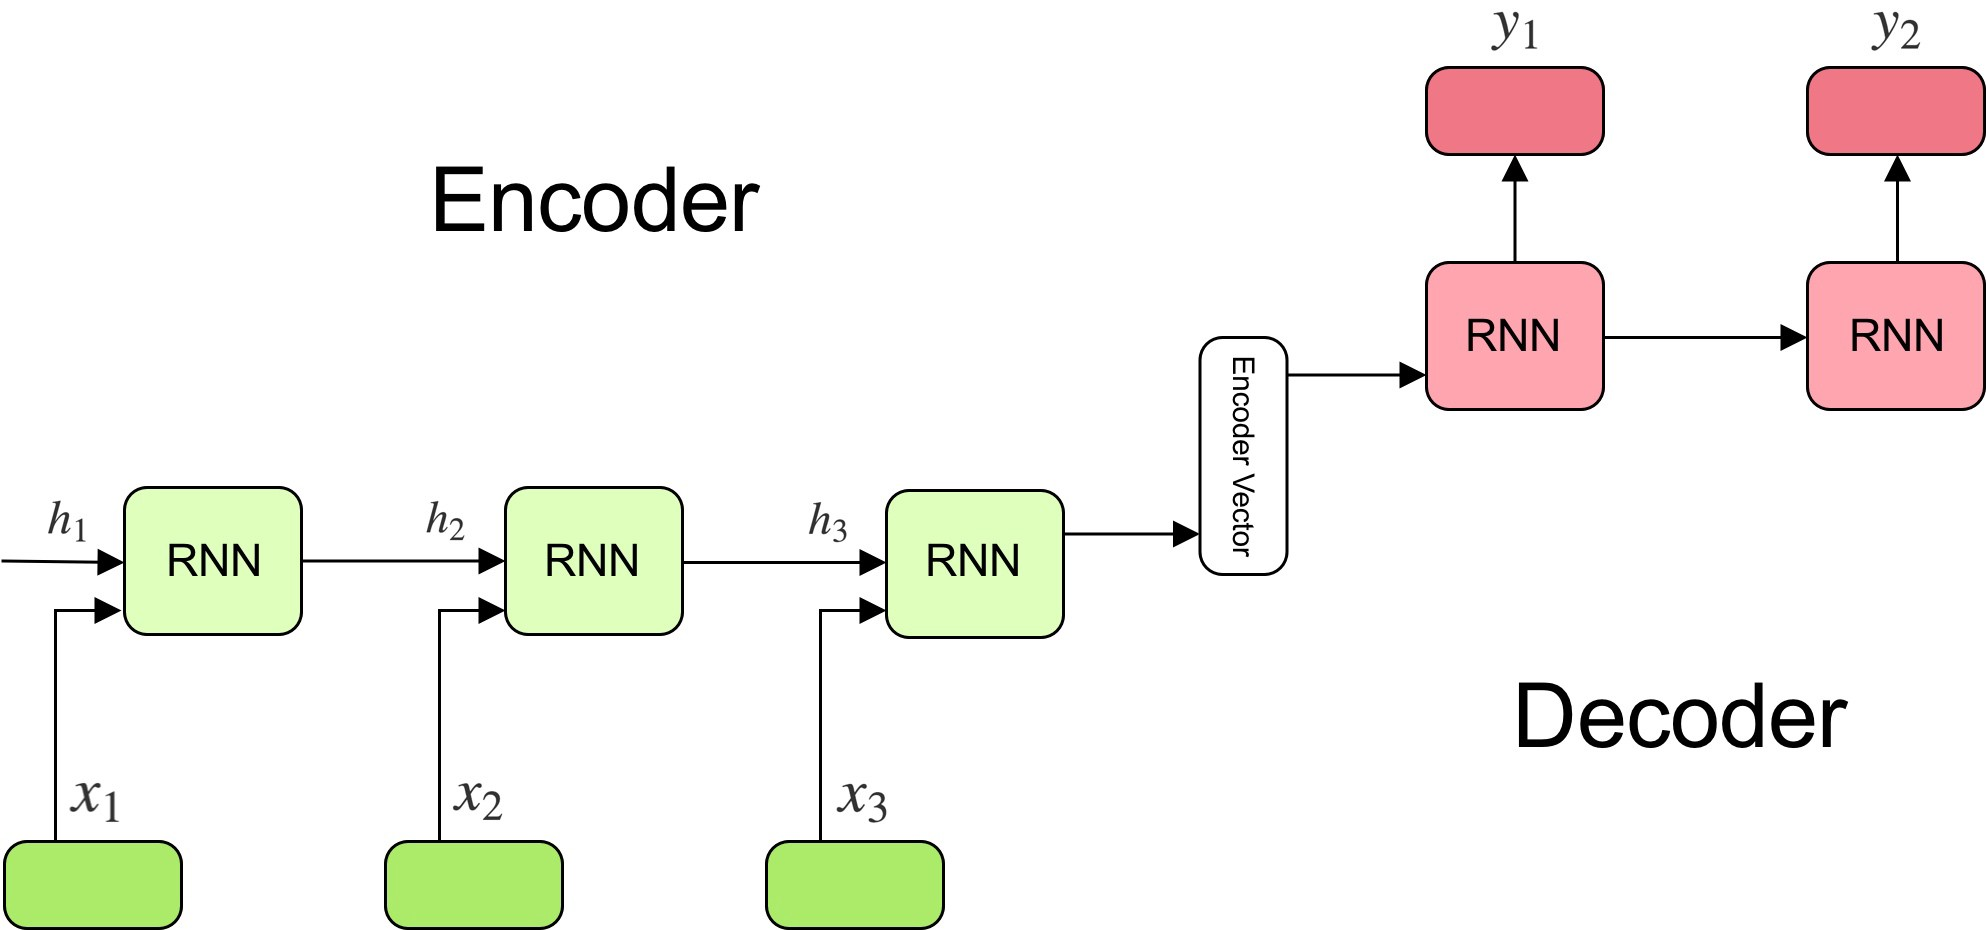
\includegraphics[width=0.45\linewidth]{Images/encoder_decoder}
		\label{fig:concatenation}
	\end{figure}
	}
\end{frame}

\begin{frame}{DNMT architectures}
	
	DNMT architectures are based on traditional encoder-decoder models:
	
	\begin{figure}
		\centering
		\textbf{Transformer-based} (afterwards)\par\medskip
		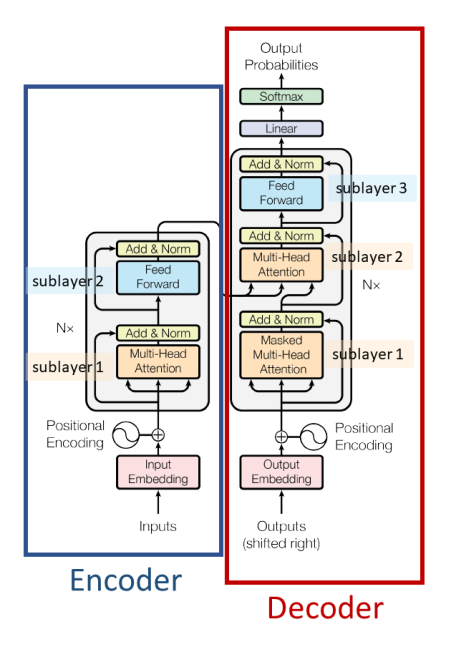
\includegraphics[width=0.3\linewidth]{Images/transformer}
		\label{fig:concatenation}
	\end{figure}
\end{frame}

%%%%%%%%%%%%%%%%%%%%%%%%%%%%%%%%%%%%%%%%%%%%%%%%%%%%%%%%%%%%%%%%%%%%%%%%%
\subsection{Concatenation Approaches}

\begin{frame}{Concatenation Approaches}
Concatenation approaches to DNMT consist in feeding a standard encoder-decoder architecture with a concatenation of sentences. 
	\begin{figure}
		\centering
		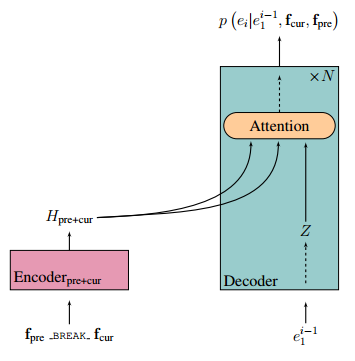
\includegraphics[width=0.45\linewidth]{Images/concatenation}
		\label{fig:concatenation}
	\end{figure}
\end{frame}

\begin{frame}{Concatenation Approaches}
For instance:
	\begin{itemize}
		\item<+(1)-|alert@+(1)> \cite{tiedemann_neural_2017} firstly introduced this approach proposing an \textbf{RNN-based} model that incorporate the preceding sentence by prepending it to the current one, separated by a $<$CONCAT$>$ token. They propose two methods:
			\begin{itemize}
				\item<+(1)-|alert@+(1)> \textbf{2-TO-2}: the previous and the current sentences are translated together. The translation of the current sentence is then obtained by only retaining the tokens following the concatenation token.
				\item<+(1)-|alert@+(1)> \textbf{2-TO-1}: only the current sentence is translated. 
			\end{itemize}
		\item<+(1)-|alert@+(1)> \cite{agrawal_contextual_2018,scherrer_analysing_2019} investigated the concatenation approach with the \textbf{Transformer} as base model, extending the number of context sentences both on the \textbf{source (s:-3,+1)} and the \textbf{target (t:-2)} side.
	\end{itemize}
\end{frame}

%%%%%%%%%%%%%%%%%%%%%%%%%%%%%%%%%%%%%%%%%%%%%%%%%%%%%%%%%%%%%%%%%%%%%%%%%
\subsection{Separate Encoding Approaches}

\begin{frame}{Separate Encoding Approaches}
Separate encoding approaches to DNMT consist in encoder-decoder models that encode the current and context sentences separately. This can be undertaken by:
	\begin{itemize}
		\item<+(1)-|alert@+(1)> \textbf{Multiple encoders} working in parallel for the current and previous sentence. E.g. \cite{wang_exploiting_2017}.
		\item<+(1)-|alert@+(1)> \textbf{Multiple encoders with shared weights}. In this case, the parallel-working encoders not only have the same architecture, but also the same weights. E.g. \cite{voita_context-aware_2018}.
		\item<+(1)-|alert@+(1)> \textbf{Two-pass approaches}, in which the encoder makes a first sentence-level encoding pass of the source, and a second in which it uses the context-agnostic drafts as contextual information for the current sentence. This can been achieved also by directly encoding the concatenation of many sentences and encoding them in a context-agnostic fashion, then encode context on top of it with extra layers. E.g. \cite{zheng_toward_2020}. See Slide \ref{slide:separateencoding}.
%		\begin{itemize}
%			\item<+(1)-|alert@+(1)> Remark: a powerful feature of two-pass approaches is their ability to exploit \textbf{future} target-side context.
%		\end{itemize}
	\end{itemize}  
\end{frame}

\begin{frame}{Separate Encoding Approaches}
Once the encoding of the current and the context sentences has been carried out, they can be integrated in different ways:
	\begin{columns}[T] % align columns
		\begin{column}{.50\textwidth}
			\begin{itemize}
				\item \textbf{Outside} the decoder. 
				\begin{itemize}
					\item (+) symbol represents a gate, a sum or a concatenation.
				\end{itemize}
			\end{itemize}
		\end{column}%
		\hfill%
		\begin{column}{.50\textwidth}
			\begin{figure}
				\centering
				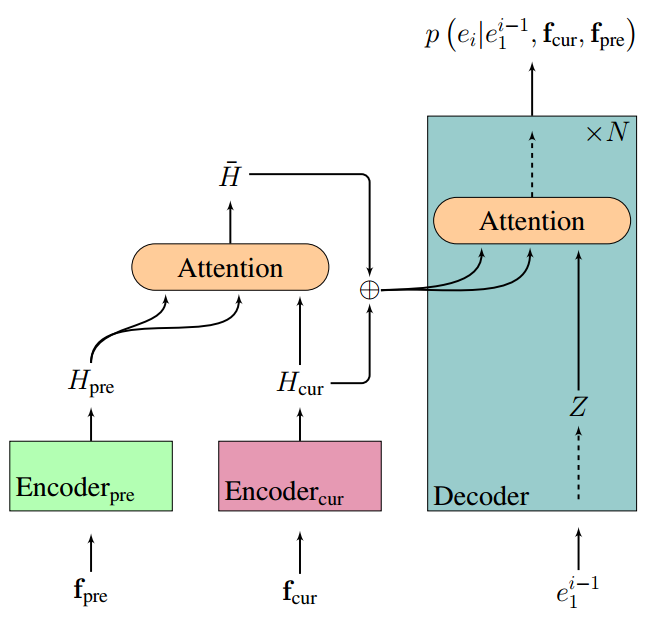
\includegraphics[width=0.90\linewidth]{Images/models_outide_decoder}
				\label{fig:modelsoutidedecoder}
			\end{figure}
		\end{column}%
	\end{columns} 
\end{frame}

\begin{frame}{Separate Encoding Approaches}
	Once the encoding of the current and the context sentences has been carried out, they can be integrated in different ways:
	\begin{columns}[T] % align columns
		\begin{column}{.50\textwidth}
			\begin{itemize}
				\item \textbf{Outside} the decoder.
					\begin{itemize}
						\item (+) symbol represents a gate, a sum or a concatenation.
					\end{itemize}
				\item \textbf{Inside} the decoder, \textbf{sequentially}. 
			\end{itemize}
		\end{column}%
		\hfill%
		\begin{column}{.50\textwidth}
			\begin{figure}
				\centering
				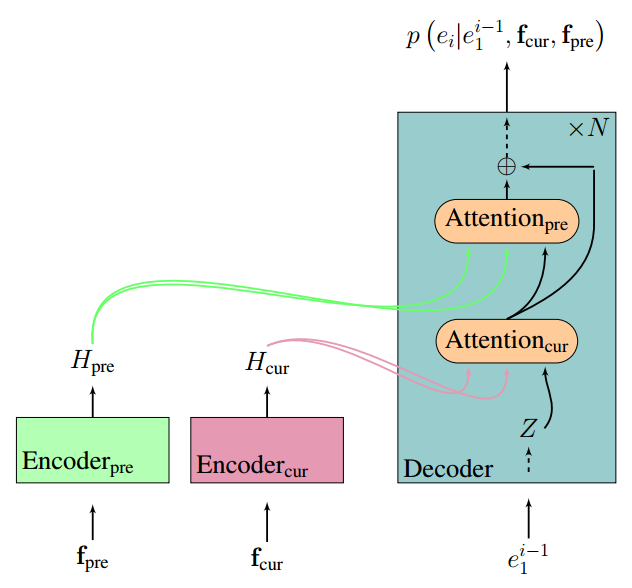
\includegraphics[width=0.90\linewidth]{Images/models_inside_decoder_sequential}
				\label{fig:modelsoutidedecoder}
			\end{figure}
		\end{column}%
	\end{columns} 
\end{frame}

\begin{frame}{Separate Encoding Approaches}
	Once the encoding of the current and the context sentences has been carried out, they can be integrated in different ways:
	\begin{columns}[T] % align columns
		\begin{column}{.50\textwidth}
			\begin{itemize}
				\item \textbf{Outside} the decoder.
					\begin{itemize}
						\item (+) symbol represents a gate, a sum or a concatenation.
					\end{itemize}
				\item \textbf{Inside} the decoder, \textbf{sequentially}.
				\item \textbf{Inside} the decoder, \textbf{in parallel}. 
			\end{itemize}
		\end{column}%
		\hfill%
		\begin{column}{.50\textwidth}
			\begin{figure}
				\centering
				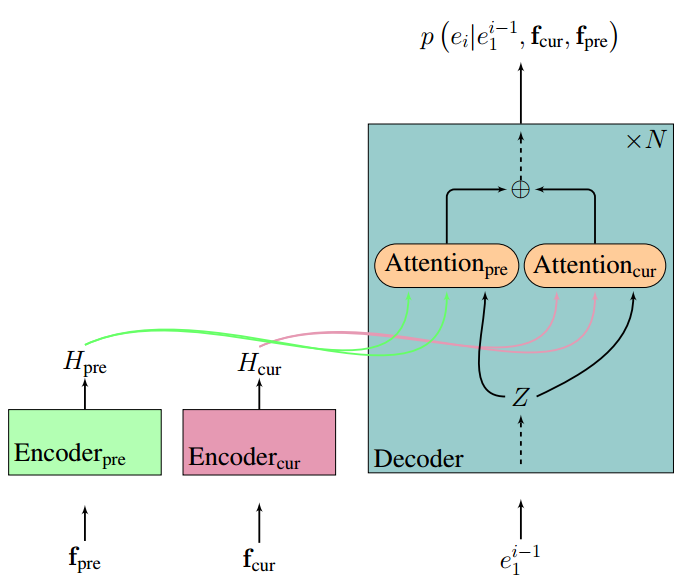
\includegraphics[width=0.90\linewidth]{Images/models_inside_decoder_parallel}
				\label{fig:modelsoutidedecoder}
			\end{figure}
		\end{column}%
	\end{columns} 
\end{frame}

%\begin{frame}{Separate Encoding Approaches}
%	\textbf{Architecture}\\
%	The encoder-decoder architectures depicted above can be both RNN-based (until 2017) or Transfomer-based (after 2017), as for any approach to DNMT. However, often some modifications are applied. For example:
%	\begin{itemize} 
%		\item<+(1)-|alert@+(1)> In the case of RNN-based architectures, integration inside the decoder can be undertaken without attention by simply concatenating context representations to the cell state of the deocdrr's RNN \cite{wang_exploiting_2017}.
%		\item<+(1)-|alert@+(1)>  Beside contextual representation of words, the context encoder can also generate higher level representations such as sentence or document embeddings. This representations can also be attended by the decoder \cite{miculicich_document-level_2018, maruf_selective_2019} or added to the word-representations \cite{tan_hierarchical_2019}.
%		\item<+(1)-|alert@+(1)> Parallel integration inside the decoder can also happen within a single multi-head attention that takes as values and queries the concatenations of the current and context sentence representations \cite{voita_when_2019}
%	\end{itemize}
%\end{frame}

\begin{frame}{Separate Encoding Approaches}
	\textbf{Including target-side context}\\
	Despite some have considered including past target-side context harmful because of the \textit{error propagation} problem \cite{zhang_improving_2018}, most recent works have showed it to be of utmost importance for making the most out of context. Past works have successfully included target-side context information in different ways:
	\begin{itemize}
		\item<+(1)-|alert@+(1)> Translating past sentences (usually 1) along with the current one, and then discarding them, as in concatenation approaches \cite{bawden_evaluating_2018}.
		\item<+(1)-|alert@+(1)> By making the decoder attend the target-side hidden representations or embeddings of previously decoded sentences \cite{miculicich_document-level_2018,voita_when_2019,maruf_selective_2019,zheng_toward_2020}.
	\end{itemize}
\end{frame}

\begin{frame}{Separate Encoding Approaches}\label{slide:separateencoding}
	\begin{table}
		\begin{tabular}{ *{5}{c|} c }

			\thead{Reference}
			& \thead{Context}
					& \thead{Two-Pass\\ Approach}
						& \thead{Outside\\ Integr.}
							& \thead{Inside\\ Integr.}
								& \thead{Lang.\\ Pair}
									 \\
			\hline\hline
			\cite{wang_exploiting_2017}&s:-3 &&aut...&...aut&Zh$\to$En\\
			\hline
			\cite{voita_context-aware_2018}&s:-1&&yes&&En$\to$Ru\\
			\hline
			\cite{zhang_improving_2018}&s:-2&&yes&sequential&Zh$\to$En\\
			\hline
			\cite{miculicich_document-level_2018}&s:-3; t:-3&&yes&&Zh/Es$\to$En\\
			\hline
			\cite{maruf_selective_2019}&s:all; t:all&optional&yes&&En$\to$De\\
			\hline
			\cite{zheng_toward_2020}&s:all; t:all&yes&yes&&Zh/En$\to$En/De\\
			\hline
			\cite{jean_does_2017}&s:-1&&&parallel&En$\to$De/Fr\\
			\hline
			\cite{bawden_evaluating_2018}&s:-1; t:-1&&&parallel&En$\to$Fr\\
			\hline
			\cite{fu_reference_2019}&s:all&yes&&parallel&En/Zh$\to$De/En\\
			\hline
			\cite{voita_when_2019}&s:-3; t:-3&yes&&parallel*&En$\to$Ru\\
			\hline
			\cite{tan_hierarchical_2019}&s:all&yes&&parallel&Zh/De$\to$En\\
			\hline
			\cite{wang_improving_2019} &s:2&&&sequential&Fr$\to$En\\
			\hline
		\end{tabular}
	\end{table}
\end{frame}

\begin{frame}{Positional Embedding Schema}
	For many approaches to DNMT, the standard positional encoding proposed by \cite{vaswani_attention_2017} is insufficient because the DNMT system needs to tell context sentences from the current one. For this reason, many strategies have been proposed in the literature, such as:
	\begin{enumerate}
		\item<+(1)-|alert@+(1)> Adding a \textbf{sentence distance embedding} to context sentences, that tell the model how far away they are from the current sentence \cite{voita_when_2019}.
		\item<+(1)-|alert@+(1)> Assign \textbf{positional embeddings progressively} to the current sentence, then to the previous one, and so on, so that far away sentences have high values of positional embedding \cite{li_pretrained_2019}.
		\item<+(1)-|alert@+(1)> Adding a \textbf{segment embedding}, similar to classical positional encoding but for the position of the sentence/segment within the document  \cite{zheng_toward_2020}.
	\end{enumerate}
\end{frame}

%%%%%%%%%%%%%%%%%%%%%%%%%%%%%%%%%%%%%%%%%%%%%%%%%%%%%%%%%%%%%%%%%%%%%%%%%
\subsection{Cache Approaches}

\begin{frame}{Cache Approaches}
	Cache approaches to DNMT consist in encoder-decoder models that are equipped with one or more caches that store context information.
	The information stored can belong to both \textbf{source side or target side, past and future}. 

	\begin{figure}
		\centering
		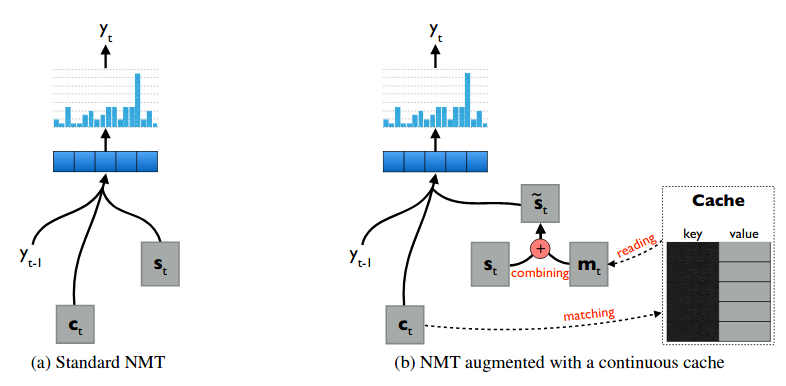
\includegraphics[width=0.7\linewidth]{Images/cache}
		\caption{Continuous cache by \cite{tu_learning_2017}}
		\label{fig:cache}
	\end{figure} 
\end{frame}

\begin{frame}[c]{Cache Approaches}
	\begin{columns}[c] % align columns
		\begin{column}{.50\textwidth}
			Every cache slot is a \textbf{key-value} tuple. With these variables, we can \textbf{read} or \textbf{write} caches.
			\vspace{0.3cm}
		\end{column}%
		\hfill%
		\begin{column}{.50\textwidth}
			\begin{figure}
				\centering
				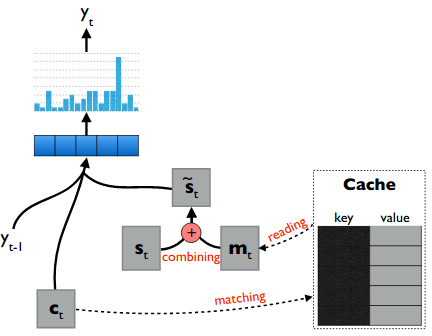
\includegraphics[width=0.9\textwidth]{Images/cache_only}
				\label{fig:cacheonly}
			\end{figure}
		\end{column}%
	\end{columns} 
\end{frame}

\begin{frame}[c]{Cache Approaches}
	\begin{columns}[c] % align columns
		\begin{column}{.50\textwidth}
			\textbf{Cache reading} involves:
			\begin{itemize}
				\item<+(1)-|alert@+(1)> Soft key matching
				\item<+(1)-|alert@+(1)> Value reading
				\item<+(1)-|alert@+(1)> Combining
			\end{itemize}
		\end{column}%
		\hfill%
		\begin{column}{.50\textwidth}
			\begin{figure}
				\centering
				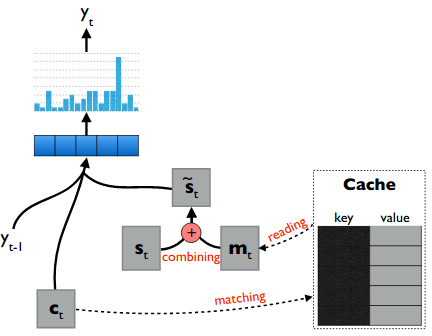
\includegraphics[width=0.9\textwidth]{Images/cache_only}
				\label{fig:cacheonly}
			\end{figure}
		\end{column}%
	\end{columns} 
\end{frame}

\begin{frame}{Cache Approaches}
	\begin{columns}[c] % align columns
		\begin{column}{.50\textwidth}
			\textbf{Cache writing} can be undertaken after having translated one or more sentences. For every triplet:
			\begin{itemize}
				\item<+(1)-|alert@+(1)> If the \textbf{key} already exists in the cache, we just update its value.  
				\item<+(1)-|alert@+(1)> Else, we write the key-value tuple in an empty slot, after having emptied the oldest slot if the cache is full.
			\end{itemize} 
		\end{column}%
		\hfill%
		\begin{column}{.50\textwidth}
			\begin{figure}
				\centering
				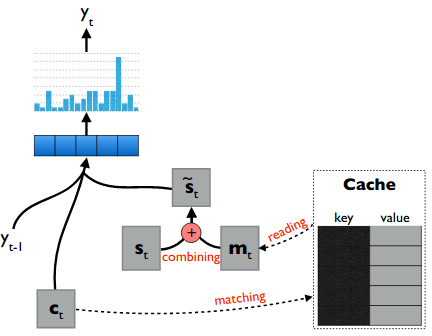
\includegraphics[width=0.9\textwidth]{Images/cache_only}
				\label{fig:cacheonly}
			\end{figure}
		\end{column}%
	\end{columns} 
\end{frame}

\begin{frame}{Cache Approaches}
	\begin{table}\small
	\begin{tabular}{p{3.6cm}|*{5}{c|} c }
		
		\thead{Reference}
		& \thead{Caches}
			& \thead{Size}
				& \thead{Key\\ (Indic.)}
					& \thead{Value}
							& \thead{Lang.\\ Pair}
		\\
		\hline\hline
		\cite{tu_learning_2017}&single&$\leq$ 500&$c_t$( $y_{k<t}$)&$s_{k<t}$&Zh$\to$En\\
		\hline
		\cite{kuang_modeling_2018}&\thead{dynamic\\ topic}&\thead{100\\ 200}&$c_t$&\thead{$y_{k<t}$\\ topic emb.}&Zh$\to$En\\
		\hline
		\cite{maruf_document_2018}&\thead{source\\ target}&\thead{doc.size}&\thead{$h_t$\\ $s_t$}&\thead{$sent. emb.$\\ $s_{k<t}$}&Fr/De/Et$\to$En\\
		\hline
	\end{tabular}
	\end{table}
\end{frame}

%%%%%%%%%%%%%%%%%%%%%%%%%%%%%%%%%%%%%%%%%%%%%%%%%%%%%%%%%%%%%%%%%%%%%%%%%
\subsection{Exploiting Document-level Monolingual Corpora}

\begin{frame}{On Parallel Corpora for Training}
	DNMT systems require training on \textbf{document-level parallel corpora}. These corpora are usually released during workshops on machine translation like IWSLT and WMT, and hosted on open source web inventories. The most common ones, are extracted from:
	\begin{itemize}
		\item<+(1)-|alert@+(1)> Movie subtitles (OpenSubtitles)
		\item<+(1)-|alert@+(1)> TED talks (WIT3)
		\item<+(1)-|alert@+(1)> News articles (LDC)
		\item<+(1)-|alert@+(1)> Parliamentary interventions (Europarl)
	\end{itemize}
\end{frame}

\begin{frame}{On Parallel Corpora for Training}
	\begin{itemize}
		\item<+(1)-|alert@+(1)> Unfortunately, document-level parallel \textbf{corpora are often insufficient} to train DNMT systems from scratch, although it is often possible to make them converge to a local optimum. 
		\item<+(1)-|alert@+(1)> \cite{kim_when_2019, li_does_2020} pointed out that when constraining training on such small datasets, model comparison becomes misleading because gains in performance are mainly related to better regularization.
		\item<+(1)-|alert@+(1)> A popular solution to this problem is the \textbf{two-step training strategy}: \cite{tu_learning_2017,zhang_improving_2018,miculicich_document-level_2018}
		\begin{enumerate}
			\item<+(1)-|alert@+(1)> Distinguish two integrated components in your model with params $\Theta=[\theta_S;\theta_D]$:
				\begin{itemize}
					\item<+(1)-|alert@+(1)> A self-standing sentence-level NMT system with parameters $\theta_S$.
					\item<+(1)-|alert@+(1)> Some context-handling modules with parameters $\theta_D$.
				\end{itemize}
			\item<+(1)-|alert@+(1)> Train $\theta_S$ independently on a sentence-level parallel corpus $C_S$.
			\item<+(1)-|alert@+(1)> Train $\theta_D$ on a document-level parallel corpus $C_D$ while fine-tuning $\theta_S$, or freezing them \cite{zhang_improving_2018}.
		\end{enumerate}
	\end{itemize}
\end{frame}

\begin{frame}{Exploiting Document-level Monolingual Corpora}
	Another solution to the lack of vast document-level parallel corpora is leveraging on huge \textit{monolingual} document-level corpora like BookCorpus \cite{zhu_aligning_2015} and PG-19 \cite{rae_compressive_2019}. In the literature, we can find various approaches to leverage monolingual corpora:
	\begin{itemize}
		\item<+(1)-|alert@+(1)> \textbf{Back-translate} target-side corpus to augment dl corpus \cite{sugiyama_data_2019}.
		\item<+(1)-|alert@+(1)> Train \textbf{context-aware language models} on target/source-side corpus, then:
		\begin{itemize}
			\item<+(1)-|alert@+(1)> Generate translations by fusioning the decoder and the LM's scores to candidate words  \cite{martinez_garcia_context-aware_2019}.
			\item<+(1)-|alert@+(1)> Initialize the econder (or decoder) of a DNMT model \cite{li_pretrained_2019}.
		\end{itemize}  
		\item<+(1)-|alert@+(1)> Train \textbf{Automatic Post Editing} systems on target-side corpus (See next slide).
	\end{itemize}
\end{frame}

\begin{frame}{Exploiting Document-level Monolingual Corpora}
	\textbf{Automatic Post Editing} (APE)\\
	\cite{voita_context-aware_2019} devised an APE system called DocRepair, that turns a sentence-level translation into a context-aware translation. DocRepair can work on top of whatever sentence-level MT system.
\end{frame}

\begin{frame}{DocRepair}
	\begin{columns}[c] % align columns
		\begin{column}{.50\textwidth}
			\begin{figure}
				\centering
				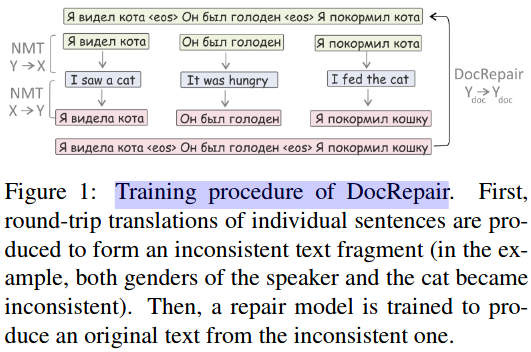
\includegraphics[width=\linewidth]{Images/docrepair_train}
				\label{fig:docrepairtrain}
			\end{figure}
		\end{column}%
		\hfill%
		\begin{column}{.50\textwidth}
			\begin{figure}
				\centering
				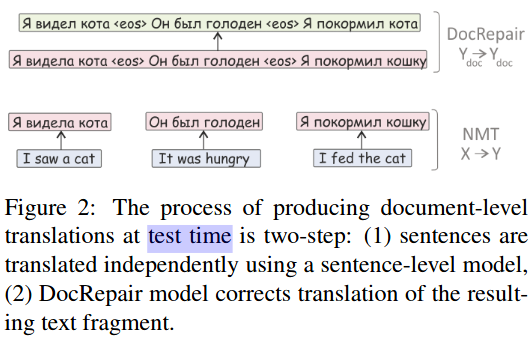
\includegraphics[width=\textwidth]{Images/docrepair_test}
				\label{fig:docrepairtest}
			\end{figure}
		\end{column}%
	\end{columns} 
\end{frame}

%%%%%%%%%%%%%%%%%%%%%%%%%%%%%%%%%%%%%%%%%%%%%%%%%%%%%%%%%%%%%%%%%%%%%%%%%
\subsection{Others}

\begin{frame}{Others}
	\textbf{Approaches Including Additional Discourse Information as Input}\\
	These approaches consist in concatenation approaches or separate encoding approaches that also integrate discourse-related information as additional input features. Examples of extra features are:
	\begin{itemize}
		\item<+(1)-|alert@+(1)> Lexical chains of semantically similar words to promote word sense disambiguation \cite{rios_gonzales_improving_2017}.
		\item<+(1)-|alert@+(1)> Coreference chains to promote coreference resolution \cite{stojanovski_coreference_2018, ohtani_context-aware_2019}.
	\end{itemize}
\end{frame}

\begin{frame}{Others}
	\textbf{Learning Approaches}\\
	 \cite{jean_context-aware_2019} looked at the problem from a learning perspective and designed a regularisation term
to encourage a DNMT model to exploit the additional context in a useful way . This regularisation
term is applied at the token, sentence and corpus levels and is based on pair-wise ranking loss,
that is, it helps to assign a higher log-probability to a translation paired with the correct context
than to the translation without context.
\end{frame}

%%%%%%%%%%%%%%%%%%%%%%%%%%%%%%%%%%%%%%%%%%%%%%%%%%%%%%%%%%%%%%%%%%%%%%%%%
\subsection{Remarks and conclusions}

\begin{frame}{Remarks and conclusions}
	\textbf{Possible Future Research Directions}
	\begin{itemize}
		\item<+(1)-|alert@+(1)> Build a large DL corpus for training systems, or find automatic approaches to generate synthetic data other than back-translation.
		\begin{itemize}
			\item<+(1)-|alert@+(1)> E.g. imputing context sentences \cite{jean_fill_2019}.
		\end{itemize}
%		\item<+(1)-|alert@+(1)> Design models with good results on lexical cohesion \cite{voita_when_2019}.
		\item<+(1)-|alert@+(1)> Design models exploiting full context in a memory-efficient way:
		\begin{itemize}
			\item<+(1)-|alert@+(1)> Dynamic context integration.
			\item<+(1)-|alert@+(1)> Caches integrated to Transformer-based models.
		\end{itemize}
		\item<+(1)-|alert@+(1)> Design automatic post-processing models that are lightweight and can be trained on little data \cite{kim_when_2019}.
		\item<+(1)-|alert@+(1)> Study pre-trained language models for DNMT decoder.
		\item<+(1)-|alert@+(1)> Study other learning methods that foster document-level modeling \cite{jean_context-aware_2019}.
	\end{itemize}
\end{frame}